\chapter{基于联邦学习与深度强化学习的并发感知任务层计算卸载方法}
\label{chap:fl_dqn_merged}

第三章已经从系统层构建了基于分层联盟链的可信协同资源分配框架，解决了多节点之间的状态共享、信誉约束与全局协调问题；但在真实运行环境中，系统层的“可协同”并不天然等价于任务层的“可高效”。当新的计算任务到达卫星终端（Satellite Terminal, ST）时，节点必须在极短时间内综合本地资源状态、链路质量、候选卫星边缘节点（Satellite Edge Node, SEN）的公共摘要以及潜在并发风险，判断应当本地执行还是卸载到哪个目标节点。若仍采用“候选节点只要当前负载不高就可安全接收任务”的静态假设，便会忽略多任务并发条件下 CPU 时间片、缓存、内存带宽和 I/O 队列竞争所带来的额外性能损失，从而使看似合理的卸载动作在实际执行中出现明显的时延放大和能耗偏差。

围绕上述问题，本章以天基分布式计算系统为研究对象，聚焦多任务并发条件下的任务级卸载决策机制，重点回答以下问题：在链上状态存在时滞、节点数据难以集中共享且样本分布明显异构的条件下，如何有效感知候选节点的并发开销，并将这种感知能力转化为节点侧可实时执行的卸载策略。为此，本文构建了“联邦学习预测 + 深度强化学习决策”的闭环方法：首先利用聚类式联邦学习在不上传原始执行日志的前提下训练并发开销预测模型，以获得对候选节点未来拥塞风险的先验估计；随后将预测结果与本地观测状态、链上公共摘要共同输入深度 Q 网络（Deep Q-Network, DQN）代理，实现节点侧实时、低开销且具备并发感知能力的任务卸载。

从章节组织上看，本章首先阐述研究背景、核心挑战和技术路线；随后给出系统场景、并发开销与任务层代价模型；在此基础上，介绍基于联邦学习的并发开销预测方法及其可信维护机制；接着给出 FL-DQN 卸载决策算法设计、在线执行流程与复杂度分析；最后通过预测精度、端到端性能、鲁棒性和消融实验验证所提方法的有效性。通过上述安排，本章形成了从问题提出、理论建模、算法设计到实验验证的完整论述链条。

从章节贡献角度看，本章的创新点可概括为四个方面：其一，面向多任务并发场景建立任务级并发开销形式化模型，将新任务进入成本与存量任务受扰成本统一纳入建模；其二，构建分层聚类联邦学习框架，在 Non-IID 与隐私受限条件下训练并发开销预测模型，并结合联盟链完成模型版本可信维护；其三，提出 FL-DQN 卸载决策机制，将并发开销预测值与置信信息显式融入状态空间和代价约束，使节点侧策略具备并发风险前瞻能力；其四，通过预测层、端到端性能、鲁棒性和消融实验的分层验证，说明所提方法在高并发和链上状态滞后条件下仍具有稳定优势。上述四点共同构成了本章相对于第三章的任务层补充，也使全文形成“系统层可信协同—任务层实时执行”的完整闭环。

\section{引言}
\label{sec:problem_statement}

随着在轨试验、遥感预处理、异常事件检测与应急响应等业务不断向天基网络侧延伸，卫星终端不再只是数据采集与转发节点，而逐步演化为具备本地处理与协同计算能力的智能边缘实体。然而，受星载平台体积、功耗、抗辐照设计和载荷预算等因素限制，卫星终端可用计算资源仍然十分有限。当计算密集型、时延敏感型任务持续到达时，仅依赖终端本地执行往往难以同时满足实时性、能耗约束与任务完成质量要求。因此，将任务动态卸载至具备更强处理能力的卫星边缘节点（Satellite Edge Node, SEN），已成为提升天基分布式计算效率的重要途径。

但对天基网络而言，真正困难的并不是“是否存在可卸载节点”，而是“面对动态环境时，节点应当如何做出正确卸载动作”。当一个新任务到达卫星终端（Satellite Terminal, ST）时，终端必须在极短时间内综合任务计算量、输入规模、时延阈值、本地资源余量、链路可达性以及候选节点状态等多维因素，判断应当本地执行，还是卸载到哪一个目标 SEN。与地面有线或稳定无线环境不同，天基网络中的链路带宽、传播时延和可见窗口随轨道运动持续变化，节点状态感知具有天然时滞，因此这一决策问题呈现出显著的动态性、局部性与不完全信息特征。

现有不少任务卸载与资源调度方法默认调度器能够获得候选节点准确、即时且全局一致的运行状态，并在此基础上进行最优动作选择。然而，这种“全局实时透明信息”假设在天基网络环境下通常难以成立。一方面，星间链路传播时延明显，链路窗口有限，节点间状态同步天然存在异步性；另一方面，不同节点的硬件能力、任务组合和负载模式存在显著差异，即便能够周期性交换状态，也难以获得足够细粒度且完全实时的系统全貌。因此，若仍采用依赖完美状态信息的集中式思路，实际部署时往往会面临观测滞后、通信开销高以及模型泛化能力不足等问题。

在上述因素中，并发开销是最容易被低估、却又最直接决定卸载效果的关键变量。当多个任务在同一候选 SEN 上并发执行时，新任务的进入不仅会延长自身完成时延，还会通过 CPU 时间片争用、缓存冲突、内存带宽竞争和 I/O 排队等机制干扰既有任务的推进过程，进而造成整个执行队列的系统级性能退化。也就是说，并发开销并不是附着于新任务本身的单一额外代价，而是同时作用于新任务与存量任务的耦合扰动。如果卸载策略仍主要依据候选节点当前平均负载、瞬时 CPU 利用率或链上静态摘要做出判断，就很容易把任务送往“表面空闲、实际拥挤”的目标节点，最终导致时延放大、能耗增加和拥塞累积。

从全文研究链条来看，第三章重点解决的是系统层面的可信协同问题，即多节点之间如何在联盟链支撑下实现状态共享、信誉约束与资源协调；而本章进一步聚焦于任务层面的实时执行问题，即在既有可信共享基础上，节点如何把链上信息转化为面向当前时刻的可执行动作。两章由此构成从{系统层可信协同}到{任务层快速决策}的连续逻辑。需要特别指出的是，联盟链在本章中的角色并不是提供某一时刻绝对精确的瞬时全局状态，而是维护一种{可信但非实时}的公共摘要：它能够保证候选节点摘要、任务生命周期事件以及模型版本信息的可验证性与一致性，却不能消除传播、确认与同步带来的时滞。因此，节点侧卸载决策不能简单依赖链上信息本身，而必须进一步结合本地观测与风险预测能力。

进一步看，在天基网络中直接沿用传统集中式训练或集中式调度思路并不可行。任务执行日志、运行轨迹和资源利用信息往往携带敏感业务特征，不适合长期集中上传；星间链路带宽有限且可用性随轨道变化波动，持续传输原始样本代价高昂；不同节点又普遍存在明显的 Non-IID 数据分布，使得统一集中模型难以稳定泛化。表~\ref{tab:centralized_limitations} 对集中式思路在本场景中的主要局限进行了总结。

\begin{table}[H]
    \centering
    \caption{集中式学习在天基网络中的主要局限}
    \label{tab:centralized_limitations}
    \begin{tabular}{p{2.3cm}p{7.2cm}p{2.6cm}}
        \toprule
        问题维度  & 具体表现                       & 直接影响      \\
        \midrule
        数据隐私  & 任务日志、运行时轨迹及资源占用明细不适合长期集中上传 & 降低可部署性    \\
        通信带宽  & 星间链路带宽有限，持续传输原始样本代价高       & 增加训练成本    \\
        链路时延  & 星地/星间传播时延明显，集中同步存在先天滞后     & 难以在线更新    \\
        链路可用性 & 卫星运动导致链路存在窗口限制和随机中断        & 影响训练稳定性   \\
        数据异构性 & 不同节点硬件能力、业务形态和负载模式差异显著     & 集中式模型泛化受限 \\
        \bottomrule
    \end{tabular}
\end{table}

基于上述约束，本章采用“并发开销预测 + 在线卸载决策”的闭环思路来解决天基任务级卸载问题：首先利用聚类式联邦学习在不上传原始执行日志的前提下训练并发开销预测模型，以学习候选节点在不同任务组合、不同运行背景下的潜在拥塞风险；随后将预测得到的并发开销及其置信信息，与任务特征、本地观测状态和链上公共摘要共同输入深度 Q 网络（Deep Q-Network, DQN）代理，生成节点侧可实时执行的离散卸载动作。之所以采用这种“预测—决策”分层结构，是因为并发开销同时受硬件架构、任务类型和执行上下文影响，用固定解析公式往往难以稳定刻画，而数据驱动的预测模型更适合学习这类复杂耦合关系；与此同时，天基任务卸载的候选动作集合通常有限，基于离散动作空间的 DQN 能够在保持较低在线推理开销的同时，将预测先验有效转化为可部署的决策能力。

据此，本章的总体目标可以概括为：在隐私受限、观测不完全、链上状态存在滞后且负载动态变化的条件下，构建一种能够显式感知并规避并发风险的任务级卸载方法，使节点侧策略在任务完成时延、能耗、吞吐量与负载均衡之间实现更合理的折中。围绕这一目标，本文主要开展以下四方面工作：第一，建立面向节点侧实时决策的任务层代价模型，将时延、能耗与并发开销统一纳入优化框架；第二，设计聚类式联邦学习机制，在 Non-IID 与隐私受限条件下训练并发开销预测模型，并通过联盟链维护模型版本可信性；第三，提出 FL-DQN 卸载决策机制，将并发开销预测值及其不确定性显式融入状态空间和代价约束设计，使智能体具备并发风险前瞻能力；第四，通过预测层、端到端性能层、鲁棒性与消融实验的分层验证，检验预测先验能否切实转化为节点侧卸载性能提升。

从实现链路看，系统在离线阶段依托历史执行日志构造并发开销监督样本，并完成聚类联邦训练与模型聚合；在在线阶段，每当新任务到达，卫星终端首先提取任务属性并采集本地状态，然后读取链上维护的候选节点公共摘要，调用目标节点所属簇的最新预测模型估计各候选动作的并发开销，最后由 DQN 输出本地执行或目标节点卸载动作。由此形成“后台训练、前台推理、链上维护可信摘要”的运行机制。按照这一逻辑，第 4.2 节将给出系统框架与任务层卸载问题建模，第 4.3 节介绍基于联邦学习的并发开销预测方法，第 4.4 节给出 FL-DQN 卸载决策算法设计，第 4.5 节通过实验验证所提方法的有效性，并在本章结尾完成阶段性总结。

\section{系统框架与任务层卸载问题建模}
\label{sec:modeling}
本节首先介绍天基分布式计算系统中的任务级卸载场景及综合代价模型，随后围绕并发开销给出形式化建模与工程近似表达，最后构造状态表征并建立任务层卸载问题的 MDP 表达，为后续联邦预测与强化决策提供统一数学基础。

\subsection{系统组成、工作流程与综合代价模型}

本节围绕天基分布式计算环境中的参与者、信息流和任务生命周期展开说明，并在此基础上引入综合代价模型。考虑由若干卫星终端 ST、卫星边缘节点 SEN、联盟链控制平面以及联邦协调单元共同构成的天基计算系统：终端节点负责业务接入、本地状态采样与卸载动作执行；边缘节点负责外部任务的接收、排队和执行；联盟链负责维护候选节点公共摘要、任务开始/结束事件以及模型版本摘要；联邦协调单元则负责预测模型的簇划分、参数聚合与版本下发。这样的角色划分使本章方法既能继承第三章提供的可信共享能力，又能在节点侧保留足够轻量的实时决策机制。

图~\ref{fig:system_framework} 给出了任务层卸载方法的系统级双闭环架构。为了避免将该图误读为单次 DQN 动作选择流程，这里先对图中两类编号作出说明：图中数字 1--5 描述的是在线任务卸载链路，即终端完成账本检查、模型版本更新、任务卸载、任务计算和任务结束上链；字母 a--e 描述的是后台联邦模型维护链路，即初始模型分发、本地模型训练、模型聚合、模型更新和区块上链。二者在时间尺度上并不相同：前者面向单任务到达后的毫秒级或秒级快速决策，后者面向历史执行日志驱动的异步模型更新。由此，图~\ref{fig:system_framework} 的作用是说明系统中“可信摘要维护、联邦预测更新和任务卸载执行”的协同关系，而后文图~\ref{fig:closed_loop} 才进一步聚焦单个任务到达后的 FL-DQN 在线决策闭环。

\begin{figure}[H]
    \centering
    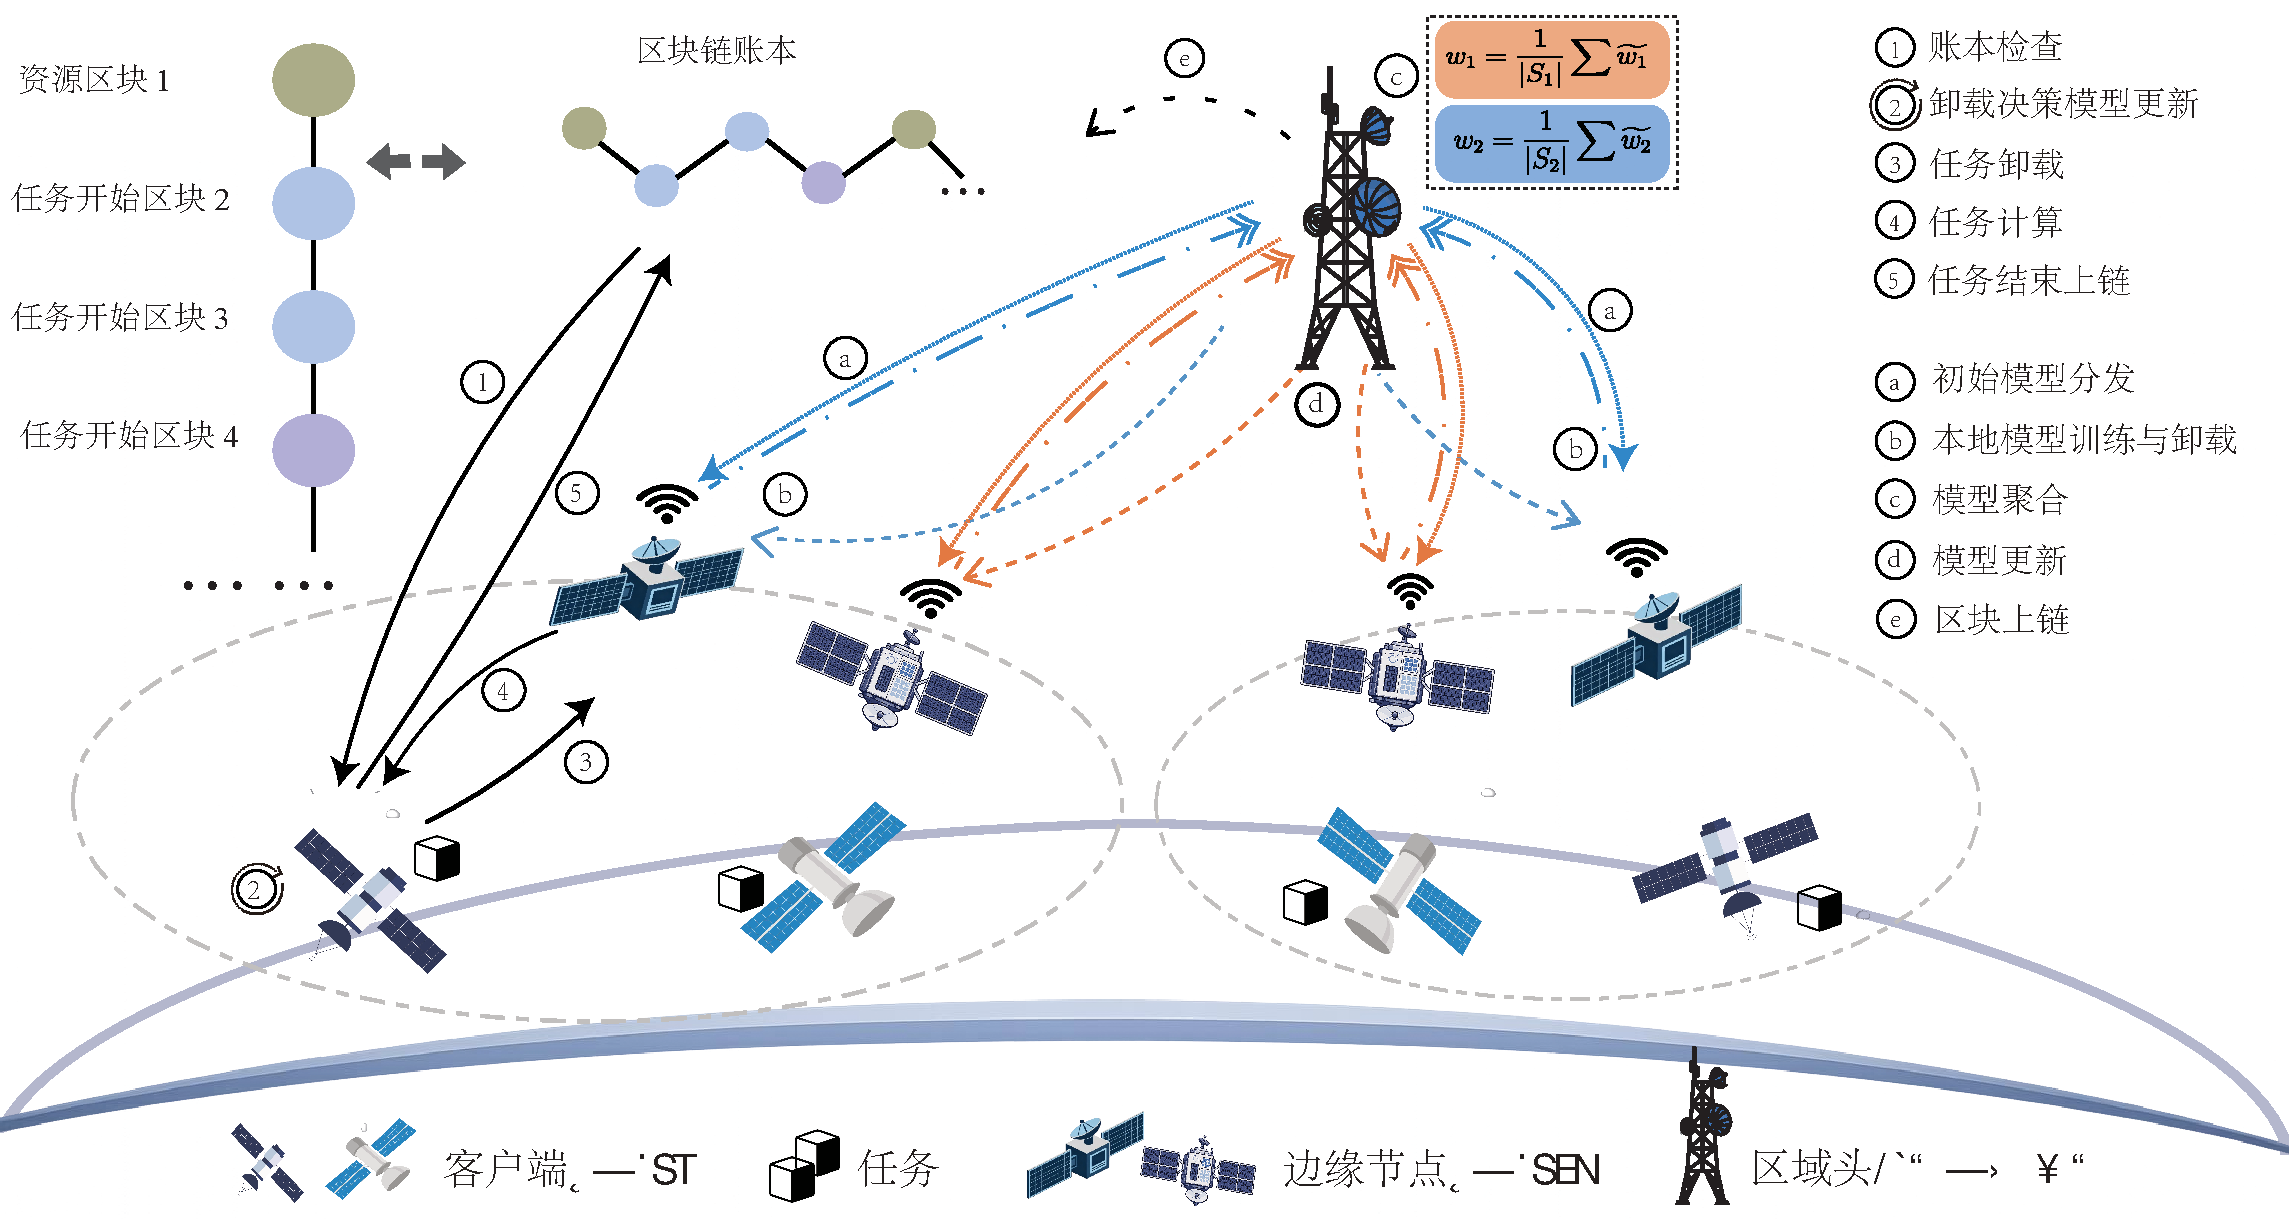
\includegraphics[width=0.95\textwidth]{figures/4-2.pdf}
    \caption{任务级卸载的系统级双闭环架构与信息交互流程}
    \label{fig:system_framework}
\end{figure}

在该系统级架构中，联盟链并不直接替代终端执行实时卸载决策，而是提供可信但非实时的公共摘要和模型版本凭据；联邦协调单元也不直接接管任务执行，而是在后台完成预测模型的簇内聚合与可信下发。为了使系统角色更清晰，表~\ref{tab:role_division} 总结了任务级卸载框架中的主要参与者及其职责。

\begin{table}[H]
    \centering
    \caption{任务级卸载框架中的角色划分}
    \label{tab:role_division}
    \begin{tabular}{p{2.5cm}p{8.8cm}}
        \toprule
        角色         & 主要职责                                               \\
        \midrule
        卫星终端 ST    & 生成新任务、采集本地 CPU/队列/剩余能量状态、读取链上摘要、触发并发开销预测并执行本地/卸载动作 \\
        卫星边缘节点 SEN & 接收外部任务、维护执行队列、反馈任务完成状态、沉淀历史执行日志并参与联邦训练             \\
        联盟链控制平面    & 维护候选节点公共摘要、任务开始/结束事件、模型版本号与哈希摘要，提供异步非实时全局视图        \\
        联邦协调单元     & 根据负载模式进行簇划分、完成簇内聚合与异常更新筛除、下发最新预测模型                 \\
        DQN 决策代理   & 将任务特征、本地状态、链上摘要和预测先验映射为离散卸载动作，并通过经验回放持续优化策略        \\
        \bottomrule
    \end{tabular}
\end{table}

从任务生命周期看，节点侧卸载决策遵循如下闭环流程：1）新任务到达后，终端提取计算量、输入规模、截止期与优先级等属性；2）终端同步采样本地资源状态，并从联盟链读取候选节点的公共摘要；3）调用候选目标所属簇的联邦预测模型，对各候选动作对应的并发开销进行快速估计；4）将任务特征、本地观测、链上摘要和预测先验拼接为统一状态向量；5）由 DQN 输出本地执行或目标节点卸载动作；6）环境返回真实时延、能耗和任务完成结果，并反向写入经验回放池；7）任务开始/结束事件与模型版本摘要继续在链上更新，构成“决策—执行—反馈—再决策”的闭环。该流程与图~\ref{fig:system_framework} 中的系统级信息流保持一致，即先由可信共享与联邦维护提供背景支撑，再由节点侧完成面向单任务的实时决策。

对任意时刻到达终端的一个新任务，记其描述为
\begin{equation}
    T_i = \left(C_i,\, S_i,\, D_i,\, \tau_i,\, \zeta_i \right),
    \label{eq:task_tuple}
\end{equation}
其中，$C_i$ 表示任务计算量，$S_i$ 表示输入数据大小，$D_i$ 为最大可接受完成时延或截止期，$\tau_i$ 为任务类型编码，$\zeta_i$ 为任务优先级。这里使用 $D_i$ 表示时延约束，是为了避免与任务符号 $T_i$ 发生混淆。

与第三章的系统层全局建模不同，本章关注的是{单任务在到达瞬间面临的局部动作选择}。设候选动作集合为
\begin{equation}
    \mathcal{A} = \left\{0,1,2,\ldots,N_c\right\},
    \label{eq:action_set}
\end{equation}
其中，动作 $0$ 表示本地执行，动作 $n \in \{1,\ldots,N_c\}$ 表示卸载至第 $n$ 个可达候选边缘节点。节点侧决策需要在一个极短时间窗口内完成，因此策略不仅要追求高质量，还要具备较低的在线推理开销。

为支撑后续奖励函数和评价指标设计，本节先给出单任务在本地执行和边缘卸载两种情形下的时延、能耗模型。

若任务在本地执行，则其完成时延由本地等待时延和本地计算时延共同构成：
\begin{equation}
    L_i^{\mathrm{loc}}(t) = W_i^{\mathrm{loc}}(t) + \frac{C_i}{f_i^{\mathrm{loc}}(t)},
    \label{eq:local_delay}
\end{equation}
其中，$W_i^{\mathrm{loc}}(t)$ 表示任务进入本地队列后的等待时间，$f_i^{\mathrm{loc}}(t)$ 为终端在当前时刻可分配给该任务的有效计算频率。相应地，本地执行能耗可写为
\begin{equation}
    E_i^{\mathrm{loc}}(t) = \kappa_i C_i \left( f_i^{\mathrm{loc}}(t) \right)^2
    + P_i^{\mathrm{idle}} W_i^{\mathrm{loc}}(t),
    \label{eq:local_energy}
\end{equation}
其中，$\kappa_i$ 为设备有效电容系数，$P_i^{\mathrm{idle}}$ 用于近似本地等待期间的空闲维持功耗。若不考虑本地排队或等待能耗，上式可退化为常见的动态功耗模型。

若任务卸载到候选边缘节点 $n$，则其端到端完成时延可分解为上行传输时延、传播时延、边缘基础排队时延、边缘计算时延和并发扰动时延五部分，即
\begin{equation}
    L_i^{\mathrm{off}}(n,t) = \frac{S_i}{R_{i,n}^{\mathrm{up}}(t)} + d_{i,n}^{\mathrm{prop}}(t)
    + W_{n}^{\mathrm{edge}}(t) + \frac{C_i}{F_n(t)} + \Delta_i(n,t),
    \label{eq:offload_delay}
\end{equation}
其中，$R_{i,n}^{\mathrm{up}}(t)$ 为上行传输速率，$d_{i,n}^{\mathrm{prop}}(t)$ 为传播时延，$W_{n}^{\mathrm{edge}}(t)$ 为不考虑新任务扰动时目标节点已有队列造成的基础等待时间，$F_n(t)$ 为目标节点当前可用计算能力，$\Delta_i(n,t)$ 为将新任务放置到节点 $n$ 后额外产生的并发开销。该写法将“已有队列导致的常规等待”和“新任务加入后造成的资源竞争扰动”分开，有助于后续突出并发开销预测模块的作用。

相应地，卸载能耗可写为
\begin{equation}
    E_i^{\mathrm{off}}(n,t) = P_i^{\mathrm{tx}}\frac{S_i}{R_{i,n}^{\mathrm{up}}(t)}
    + P_i^{\mathrm{idle}}\left(d_{i,n}^{\mathrm{prop}}(t)+W_{n}^{\mathrm{edge}}(t)\right)
    + \eta_n \frac{C_i}{F_n(t)},
    \label{eq:offload_energy}
\end{equation}
其中，$P_i^{\mathrm{tx}}$ 为终端发射功率，$\eta_n$ 为将目标节点执行能耗折算回任务代价的系数。式~(\ref{eq:offload_energy}) 不仅刻画了传输能耗，也保留了等待和边缘侧执行的代价信息，从而避免策略一味追求低时延卸载而忽略系统整体能源消耗。

在进一步建模之前，有必要说明本章变量的来源与适用边界。任务计算量、输入数据规模、截止期和优先级来自业务层任务描述；本地 CPU 占用、队列长度、剩余能量和可用频率由终端实时采样获得；候选节点平均负载、负载方差、信誉评分和模型版本号等信息来自联盟链维护的公共摘要；执行中任务剩余工作量、上下文切换强度和资源争用统计由边缘节点日志离线统计获得，并在联邦训练阶段转化为监督样本。与此同时，式~(\ref{eq:offload_delay}) 与式~(\ref{eq:offload_energy}) 建立在几个工程假设之上：其一，任务到达可用泊松流或离散事件过程近似；其二，边缘节点在短时间窗内的标称算力变化相对平缓；其三，链上摘要虽然可能存在陈旧性，但版本顺序和摘要内容是可信的。后续实验中的链上滞后敏感性分析，正是对上述假设边界进行专门验证。

\subsection{并发开销建模}

并发开销是本章区别于传统卸载模型的关键变量。设在时刻 $t$，目标节点 $n$ 上已有执行中任务集合 $\mathcal{T}_{n}^{\mathrm{exec}}(t)$，新任务 $T_i$ 被放置到该节点后，系统会因 CPU 时间片争用、缓存冲突、内存带宽竞争和 I/O 排队而出现额外时延。为了同时刻画新任务自身被拖慢和存量任务被扰动两类影响，将任务 $T_i$ 产生的并发开销定义为
\begin{equation}
    CO_i(n,t) =
    \left[L_i^{\mathrm{conc}}(n,t)-L_i^{\mathrm{base}}(n,t)\right]
    + \sum_{e \in \mathcal{T}_{n}^{\mathrm{exec}}(t)}
    \left[\widetilde{L}_{e}^{\mathrm{conc}}(n,t)-\widetilde{L}_{e}^{\mathrm{base}}(n,t)\right],
    \label{eq:co_formal}
\end{equation}
其中，$L_i^{\mathrm{base}}(n,t)$ 表示新任务在目标节点不受额外并发扰动时的基准完成时延，$L_i^{\mathrm{conc}}(n,t)$ 表示新任务加入真实并发环境后的完成时延；$\widetilde{L}_{e}^{\mathrm{base}}(n,t)$ 表示存量任务 $e$ 在没有新任务 $T_i$ 加入时的预计剩余完成时延，$\widetilde{L}_{e}^{\mathrm{conc}}(n,t)$ 表示新任务加入后该存量任务的剩余完成时延。与只关注新任务自身时延的定义相比，式~(\ref{eq:co_formal}) 同时计入了新任务进入成本与存量任务受扰成本，因此更符合节点侧真实的资源竞争机制。

图~\ref{fig:co_illustration} 展示了并发开销的形成机理。该图应与式~(\ref{eq:co_formal}) 对应理解：左侧表示无新任务加入时存量任务按相对稳定的资源份额推进；右侧表示新任务进入后，CPU、Cache、Memory 和 I/O 等共享资源被重新分配，存量任务出现受扰延迟，新任务也因竞争产生额外等待。因而，并发开销不是单个任务的固定附加项，而是由任务组合、资源瓶颈和执行上下文共同决定的耦合代价。

\begin{figure}[H]
    \centering
    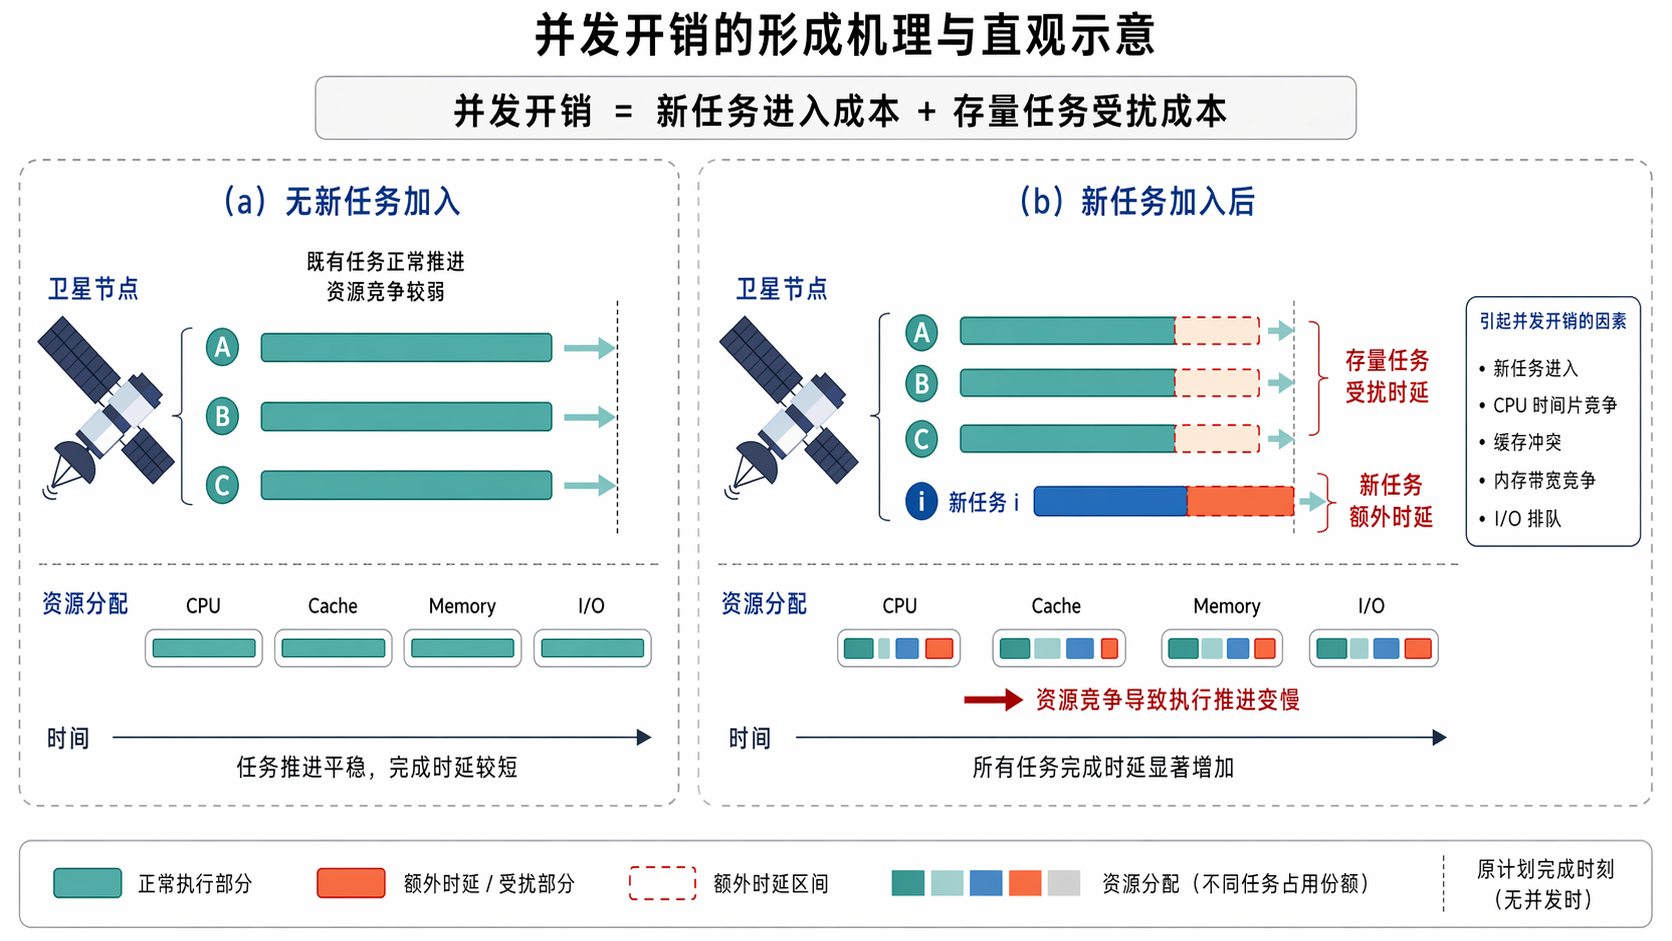
\includegraphics[width=0.92\textwidth]{figures/4-3.png}
    \caption{并发开销的形成机理与资源争用示意}
    \label{fig:co_illustration}
\end{figure}

在工程实现中，式~(\ref{eq:co_formal}) 所涉及的未来并发时延难以在决策瞬间直接获得，因此还需构造一个可学习、可预测的近似表达。记目标节点当前并发任务数为 $k_n(t)$，节点当前可用计算能力为 $F_n(t)$，执行中任务 $e$ 的剩余计算量为 $C_e^{\mathrm{rem}}(t)$，并用 $\chi_{i,e}\in[0,1]$ 表示新任务与存量任务在资源需求类型上的竞争强度，则并发扰动可近似写为
\begin{equation}
    \Delta_i(n,t) \approx \frac{\left(k_n(t)-1\right)C_i}{F_n(t)}
    + \sum_{e \in \mathcal{T}_{n}^{\mathrm{exec}}(t)}
    \frac{\chi_{i,e} C_e^{\mathrm{rem}}(t)}{F_n(t)},
    \label{eq:co_approx}
\end{equation}
该表达式揭示了并发开销与新任务计算量、当前并发任务数、存量任务剩余工作量以及任务间资源竞争强度之间的正相关关系，便于在后续样本标注、特征选择和模型解释中使用。当缺少细粒度资源画像时，可令 $\chi_{i,e}=1$ 得到保守估计。

进一步地，从统计学习角度可以将并发开销写为
\begin{equation}
    CO_i(n,t) \approx F_{\mathrm{new}}(T_i,n,\mathrm{obs})
    + G_{\mathrm{exec}}(\mathcal{T}_{n}^{\mathrm{exec}}(t),n,\mathrm{obs})
    + R_i(n,t),
    \label{eq:co_decomp}
\end{equation}
其中，$F_{\mathrm{new}}(\cdot)$ 捕获新任务加入带来的瞬时冲击，$G_{\mathrm{exec}}(\cdot)$ 刻画已执行任务间的持续资源竞争，$R_i(n,t)$ 表示未建模的高阶耦合残差。该可分解表达虽不直接用于在线推理，却有助于解释为何联邦模型在轻负载和重负载场景下会表现出不同的误差模式：前者更依赖新任务特征，后者更依赖存量任务组合和运行背景。

考虑时延、能耗和并发扰动三类代价，本章将动作 $a_t$ 对应的单任务总代价定义为
\begin{equation}
    J_i(a_t) = \omega_L L_i(a_t) + \omega_E E_i(a_t) + \omega_C \Delta_i(a_t),
    \qquad
    \omega_L+\omega_E+\omega_C=1,
    \label{eq:total_cost}
\end{equation}
其中，$L_i(a_t)$ 为动作执行后的端到端完成时延，$E_i(a_t)$ 为对应能耗，$\Delta_i(a_t)$ 表示动作引起的并发扰动；对于本地执行动作，可令 $\Delta_i(a_t)$ 表示本地队列中存量任务受到的额外扰动，也可在只关注边缘并发时取零。三个权重参数可根据业务偏好灵活调整：对实时业务可提高 $\omega_L$，对能源敏感任务可提高 $\omega_E$，对高拥塞控制场景则可适当增加 $\omega_C$。采用 $\omega$ 作为代价权重，是为了避免与后续 DQN 中的折扣因子符号混用。

值得指出的是，式~(\ref{eq:total_cost}) 的意义并不仅在于给出加权求和目标，更重要的是为后续 DQN 奖励函数设计提供统一的任务层优化视角。第三章关注的是系统层的全局资源配置，本章则将优化边界收缩到{节点侧单任务决策}，从而在保持整体方法链连贯性的同时，避免重复求解上一章已经讨论过的系统层全局资源调度问题。

\subsection{状态表征构造}

为了使并发开销能够被机器学习模型预测，并使 DQN 能够进行可执行的在线决策，需要构造一个统一的复合状态表征。设可观测特征向量为
\begin{equation}
    \bm{x} = \left[ \bm{x}^{\mathrm{task}},\,
        \bm{x}^{\mathrm{local}},\,
        \bm{x}^{\mathrm{chain}},\,
        \bm{x}^{\mathrm{conc}}
        \right],
    \label{eq:feature_vector}
\end{equation}
其中：
\begin{itemize}[leftmargin=2.5em]
    \item $\bm{x}^{\mathrm{task}}$：新任务特征，包括计算量、输入大小、时延阈值、任务类型编码、优先级等；
    \item $\bm{x}^{\mathrm{local}}$：本地状态，包括本地 CPU 占用、队列长度、剩余能量、可用频率和链路质量估计等；
    \item $\bm{x}^{\mathrm{chain}}$：链上公共摘要，包括候选节点平均负载、负载方差、信誉评分、账本确认延迟估计等；
    \item $\bm{x}^{\mathrm{conc}}$：并发环境统计，包括目标节点当前并发任务数、执行中任务总剩余工作量、平均内存占用和上下文切换强度等。
\end{itemize}

所有连续特征在进入模型前都进行标准化处理，即
\begin{equation}
    \tilde{x}_j = \frac{x_j - \mu_j}{\sigma_j + \varepsilon},
    \label{eq:normalize}
\end{equation}
其中，$\mu_j$ 和 $\sigma_j$ 分别为训练集统计均值和标准差，$\varepsilon$ 为数值稳定常数。

需要强调的是，节点侧状态天然是不完全的：一方面，本地节点只能直接观测自身状态，无法获取其他候选节点的细粒度实时运行轨迹；另一方面，链上摘要虽然提供了全网一致视图，但其时间戳可能早于当前决策时刻。因此，本章所研究的卸载问题本质上是在{部分可观测、带滞后信息的动态环境}下进行的序贯决策问题。引入 FL 预测模块的意义，正是在不可能获得完整实时信息的前提下，用历史数据学习出的风险先验来弥补观测缺口。

\subsection{任务层卸载问题的马尔可夫决策过程建模}

在上述基础上，节点侧任务卸载被建模为马尔可夫决策过程
\begin{equation}
    \mathcal{M} = \langle \mathcal{S}, \mathcal{A}, \mathcal{P}, \mathcal{R} \rangle.
\end{equation}
其中：
\begin{itemize}[leftmargin=2.5em]
    \item 状态空间 $\mathcal{S}$ 由任务特征、本地资源状态、链上公共摘要和 FL 预测值共同组成；
    \item 动作空间 $\mathcal{A}$ 为“本地执行 + 若干候选 SEN”构成的离散集合；
    \item 状态转移概率 $\mathcal{P}$ 由任务到达、链路变化、资源占用演化和预测结果更新共同决定；
    \item 奖励函数 $\mathcal{R}$ 采用总代价负值并叠加轻量奖惩项。
\end{itemize}

为了便于工程部署，本章选择基于离散动作值函数的 DQN，而没有采用连续动作策略梯度类方法，主要原因有二：其一，本场景的动作集合有限，DQN 推理效率高、实现成本低；其二，本章更希望把模型复杂度预算留给“并发开销预测”这一难点环节，而非在在线阶段引入过于复杂的连续动作网络。

\section{基于联邦学习的并发开销预测方法}
\label{sec:fl_prediction}
在上一节完成任务层代价建模之后，本节进一步回答“并发开销如何在隐私受限和样本异构条件下被有效学习”这一问题。按照“预测目标—模型结构—联邦训练—可信维护”的链式逻辑，本节首先说明监督样本如何从执行日志中构造，其次给出预测器为什么采用轻量 MLP/1D-CNN 结构，再介绍聚类式联邦训练为何优于统一 FedAvg，最后讨论模型版本如何借助联盟链进行可信维护与在线调用。这样的组织方式与参考章节中“框架概述之后再逐层展开算法设计”的写法保持一致，便于读者把每个模块放回整体系统闭环中理解。

\subsection{预测目标与样本构造}

并发开销预测本质上是一个监督回归问题。其输入为式~(\ref{eq:feature_vector}) 定义的多维特征，输出为目标节点在接受新任务后的并发开销估计值 $\widehat{\Delta}$ 及其置信信息。设节点本地构造的监督样本为
\begin{equation}
    \mathcal{D}_k = \left\{ \left(\bm{x}^{(m)}, y^{(m)} \right) \right\}_{m=1}^{N_k},
\end{equation}
其中，$y^{(m)}$ 为根据运行日志标注得到的真实并发开销。对于每个样本，需要记录任务到达前后的队列长度、CPU 频率、内存占用、任务开始时间、完成时间、输入大小、计算量等信息，再依照式~(\ref{eq:co_formal}) 或式~(\ref{eq:co_approx}) 计算标签。

为了使预测模型尽可能覆盖多样化的竞争形态，本章沿用原稿中的“双代理负载”的思路：一类是图像处理任务，用于模拟视觉感知类边缘业务；另一类是数值计算任务，用于模拟计算密集但数据规模较小的负载。这种设计的好处在于，既能让模型观察到数据搬移开销与计算开销同时占优的混合场景，又能避免训练集完全偏向单一类型任务而失去泛化性。

\subsection{预测模型结构设计}

考虑到输入特征既包含结构化统计量，也可能包含短时间窗内的序列信息，本章在模型结构上兼容两类实现：

\begin{enumerate}[label=\arabic*)]
    \item {MLP 结构}：适用于结构化向量输入。模型通常由 3--5 个全连接隐藏层构成，每层采用 ReLU 激活并可结合 Dropout 抑制过拟合；
    \item {1D-CNN 结构}：当输入拼接了过去若干时间步的 CPU 利用率、队列长度或链路质量序列时，1D-CNN 可以提取时序局部模式，再通过全连接层输出最终预测值。
\end{enumerate}

为了使预测结果能够在决策阶段发挥更稳健的作用，本章进一步采用{均值 + 方差双输出}的设计，即网络输出
\begin{equation}
    f_{\theta}(\bm{x}) = \left(\widehat{\Delta},\, \widehat{\sigma}^2 \right),
\end{equation}
其中，$\widehat{\Delta}$ 为并发开销点估计，$\widehat{\sigma}^2$ 为预测方差估计。与只输出单一标量相比，增加不确定性分支具有两方面价值：一是便于在 DQN 状态中引入“模型对该预测是否有把握”的额外信息；二是在高异构、弱覆盖样本区间内，不确定性可以提醒策略避免过度依赖单一预测值。

从实现角度看，预测器本身不追求过深或过重的网络结构，而强调对结构化特征、短时间窗统计序列以及不确定性信息的统一表达。也正因为本章的重点在于“并发风险感知如何服务任务级决策”，所以模型结构仅保留轻量、可部署和可解释的设计原则，而不将网络复杂度本身作为主要创新点。

在损失函数设计上，若仅关注点估计，可使用均方误差
\begin{equation}
    \mathcal{L}_{\mathrm{MSE}} = \frac{1}{N}\sum_{m=1}^{N}
    \left( \widehat{\Delta}^{(m)} - \Delta^{(m)} \right)^2.
    \label{eq:mse_loss}
\end{equation}
若同时训练不确定性分支，则可以采用异方差高斯负对数似然形式
\begin{equation}
    \mathcal{L}_{\mathrm{pred}}
    =
    \frac{1}{N}
    \sum_{m=1}^{N}
    \left[
        \frac{\left(\widehat{\Delta}^{(m)}-\Delta^{(m)}\right)^2}{2\widehat{\sigma}^{2(m)}}
        +
        \frac{1}{2}\log \widehat{\sigma}^{2(m)}
        \right].
    \label{eq:hetero_loss}
\end{equation}
该损失函数允许模型在噪声较大的区域给出更高的不确定性估计，从而避免对本就难以准确预测的样本过度拟合。

\subsection{分层聚类联邦架构与训练流程}

由于不同边缘卫星节点的本地样本分布具有显著 Non-IID 特征，直接使用统一的 FedAvg 训练单一全局模型往往难以兼顾不同簇之间的局部负载模式。基于此，本文采用聚类式联邦学习（clustered FL）对预测模型进行训练。其核心思路是：不再假设全网节点共享同一个最优模型，而是先根据节点负载模式、硬件能力或更新方向将其划分为多个簇，再在簇内执行模型聚合。

面向天基网络的层次化结构，本章将联邦预测框架设计为“全局协调层—区域聚合层—本地训练层”三层架构。与参考章节中“系统组成—工作流程—算法设计”的写法一致，这里先说明各层角色，再给出训练流程与簇内聚合规则。

三层架构的职责分工如表~\ref{tab:fl_roles} 所示。

\begin{table}[H]
    \centering
    \caption{分层聚类联邦学习架构中的角色划分}
    \label{tab:fl_roles}
    \begin{tabular}{p{2.7cm}p{3.0cm}p{6.0cm}}
        \toprule
        层级    & 典型实体           & 主要职责                           \\
        \midrule
        全局协调层 & 地面控制中心 / 星座控制器 & 模型版本管理、训练轮次调度、簇级模型下发、链上摘要维护    \\
        区域聚合层 & 核心边缘卫星节点       & 区域内节点分组、异常更新检测、簇内参数加权聚合        \\
        本地训练层 & 参与训练的 SEN 集合   & 基于本地执行日志训练预测模型，不上传原始样本，仅上传模型更新 \\
        \bottomrule
    \end{tabular}
\end{table}

在一次完整的联邦训练周期内，预测模型的工作流程可以概括为：1）全局协调层根据节点历史负载模式完成簇划分并下发初始化模型；2）本地训练层在各自执行日志上完成若干轮本地更新；3）区域聚合层对上传参数执行一致性检查、异常更新筛除与簇内加权聚合；4）聚合后的模型版本号和参数哈希写入联盟链，供后续在线推理时进行版本校验与追溯；5）最新簇模型再次下发至簇内节点，进入下一轮训练。上述流程使预测模型的训练、维护和可信存证形成统一闭环。

设第 $c$ 个簇内包含若干节点集合 $C_c$，第 $t$ 轮通信后簇模型参数更新为
\begin{equation}
    \theta_c^{(t+1)} =
    \sum_{k \in C_c}
    \frac{n_k}{\sum_{j \in C_c}n_j}
    \theta_k^{(t+1)},
    \label{eq:cluster_fedavg}
\end{equation}
其中，$n_k$ 为节点 $k$ 的本地样本量，$\theta_k^{(t+1)}$ 为节点本地更新后的参数。与传统 FedAvg 相比，式~(\ref{eq:cluster_fedavg}) 的改进并不体现在加权形式本身，而在于聚合只在“样本分布相近的节点簇内”进行，因此更容易捕捉局部任务模式。

在实现层面，聚类式联邦训练不只是“把 FedAvg 换成簇内 FedAvg”，还需要把训练过程与区块链提供的可信机制结合起来。具体而言，区域聚合层在每轮簇内聚合后，可将模型版本号、参数哈希和训练轮次摘要写入联盟链，用于完成模型溯源、版本一致性校验与异常更新留痕；终端节点在调用预测器时只需读取候选节点当前所属簇的最新可用模型版本，从而避免在在线阶段访问原始训练日志。这样的设计使“数据不出域”和“模型可追溯”同时成立，也使预测模块更容易并入第三章已经建立的可信协同框架中。

聚类式联邦学习的一个完整训练轮次可由算法~\ref{alg:clusterfedavg} 概括。相较原始 FedAvg，该流程新增了簇内聚合、异常更新筛查与链上存证三个关键步骤，因此更适合 Non-IID 且可信要求较高的天基边缘场景。

\begin{algorithm}[H]
    \caption{聚类式联邦学习（Clustered FedAvg）训练流程}
    \label{alg:clusterfedavg}
    \small
    \begin{algorithmic}[1]
        \Statex {输入：}簇划分集合 $\{C_1,\ldots,C_K\}$，本地数据集 $\mathcal{D}_k$，本地训练轮数 $E$，通信轮数 $T$。
        \Statex {输出：}各簇最终预测模型参数 $\theta_c^{(T)}$。
        \For{每个簇 $C_c$}
        \State 初始化簇模型参数 $\theta_c^{(0)}$ 并下发至簇内节点
        \EndFor
        \For{$t=0,1,\ldots,T-1$}
        \For{每个簇 $C_c$ 并行执行}
        \For{每个参与节点 $k\in C_c$}
        \State 以 $\theta_c^{(t)}$ 为初值，在 $\mathcal{D}_k$ 上执行 $E$ 个 epoch 本地更新
        \State 得到本地参数 $\theta_k^{(t+1)}$ 及样本量 $n_k$
        \EndFor
        \State 区域聚合层对上传更新做一致性检查与异常筛除
        \State 按式~(\ref{eq:cluster_fedavg}) 聚合得到新的簇模型 $\theta_c^{(t+1)}$
        \State 将模型版本号、参数哈希及训练轮次摘要写入联盟链
        \EndFor
        \EndFor
    \end{algorithmic}
\end{algorithm}

在线推理阶段，终端节点并不直接参与联邦训练，而是在需要决策时调用候选边缘节点所属簇的最新预测模型，对每个候选动作的并发开销进行快速估计。这一点十分重要：联邦学习的高开销发生在离线训练或后台异步更新阶段，而在线阶段保留下来的只是一个轻量前向推理过程，因此不会破坏节点侧决策的实时性要求。

\subsection{可信维护与复杂度分析}

从时间复杂度看，若单个本地预测模型包含 $P_f$ 个参数，本地每轮训练使用 $B_f$ 个 mini-batch，则节点单轮本地训练复杂度约为 $\mathcal{O}(B_f P_f)$；簇内聚合本质是参数加权求和，复杂度为 $\mathcal{O}(|C_c|P_f)$。由于聚类式 FL 把全局聚合分解为多个簇内聚合过程，单轮同步对全网连通性的要求低于统一 FedAvg。相比之下，在线阶段仅保留一次前向推理，因此预测模块在部署时的主要成本不是计算本身，而是模型版本刷新与链上摘要读取的调度机制。

从通信复杂度看，联邦学习阶段每轮只需要在节点与聚合层之间传递参数摘要，而无需传递原始日志数据。在天基网络这类带宽和链路可用性受限的环境中，这种“模型移动而非数据移动”的设计具有明显优势。与此同时，聚类式 FL 还可以借助区域聚合层把大规模全局同步拆解成多个较小的局部同步过程，降低单轮训练对网络连通性的苛刻要求。

进一步地，若把模型可信维护纳入考虑，则每轮额外链上开销主要来自模型哈希写入和版本确认，这部分复杂度与模型参数规模无关，而与摘要长度和交易确认时延有关。因此，区块链并不会显著增加预测器训练的算力负担，但会通过信息年龄影响在线可用模型版本的新鲜度。后续实验中的“链上确认延迟敏感性”正是对这一现实部署约束的量化验证。

\section{FL-DQN 卸载决策算法设计}
\label{sec:dqn_policy}
如果说上一节解决的是“如何看见未来并发风险”，那么本节解决的便是“如何把这种风险感知转化为实时动作”。因此，本节不再重复描述预测模型本身，而是聚焦于节点侧决策代理如何读取预测先验、如何构造奖励约束、如何在在线阶段完成闭环交互，以及为什么该算法在工程上可实现。整体上，本节按照“状态—奖励—训练—在线执行—复杂度”的顺序展开，使算法描述与章节主线保持一致。

\subsection{状态、动作与奖励函数设计}

在获得并发开销预测能力后，节点侧仍需进一步解决“面对新任务应当本地执行还是卸载到哪个候选节点”的决策问题。本文将单个 ST 的卸载过程建模为 MDP，其状态向量定义为
\begin{equation}
    s_t =
    \left[
        s_t^{\mathrm{task}},\,
        s_t^{\mathrm{local}},\,
        s_t^{\mathrm{chain}},\,
        s_t^{\mathrm{FL}}
        \right],
    \label{eq:dqn_state}
\end{equation}
其中，$s_t^{\mathrm{task}}$ 包含任务计算量、数据规模、截止期、任务类型编码与优先级；$s_t^{\mathrm{local}}$ 包含本地 CPU 占用、队列长度、剩余能量与链路质量估计；$s_t^{\mathrm{chain}}$ 来自联盟链上的候选节点公共摘要；$s_t^{\mathrm{FL}}$ 则由并发开销预测模型给出，包括各候选动作的 $\widehat{\Delta}_i(n,t)$ 及其不确定性 $\widehat{\sigma}_i^2(n,t)$。

表~\ref{tab:state_space} 总结了复合状态空间的设计。

\begin{table}[H]
    \centering
    \caption{节点侧决策的复合状态空间设计}
    \label{tab:state_space}
    \begin{tabular}{p{3.1cm}p{5.8cm}p{3.0cm}}
        \toprule
        状态分量      & 主要内容                               & 作用            \\
        \midrule
        任务特征向量    & 任务计算量、输入数据大小、截止期、任务类型编码、优先级        & 刻画当前任务需求      \\
        本地资源与链路状态 & 本地 CPU 占用、队列长度、剩余能量、可用频率、链路时延与带宽估计 & 反映当前本地资源与通信条件 \\
        链上公共摘要    & 候选节点平均负载、负载方差、信誉评分、账本延迟估计          & 提供系统级非实时协同上下文 \\
        FL 预测先验   & 各候选动作的并发开销预测值与不确定性                 & 显式表征卸载后的额外风险  \\
        \bottomrule
    \end{tabular}
\end{table}

奖励函数在总代价负值的基础上引入轻量奖惩机制：
\begin{equation}
    r_t = -\left(
    \omega_L L_i^{\mathrm{obs}}
    + \omega_E E_i^{\mathrm{obs}}
    + \omega_C \Delta_i^{\mathrm{obs}}
    \right)
    - \lambda_b P_{\mathrm{imbalance}}
    - \lambda_u \overline{\sigma}_t
    + R_{\mathrm{succ}},
    \label{eq:reward}
\end{equation}
其中，$L_i^{\mathrm{obs}}$、$E_i^{\mathrm{obs}}$ 和 $\Delta_i^{\mathrm{obs}}$ 分别表示任务执行后观测到的真实时延、能耗和并发扰动；$P_{\mathrm{imbalance}}$ 表示负载不均衡惩罚项，用于抑制任务长期集中到少数高性能边缘节点；$\overline{\sigma}_t$ 表示当前被选动作或候选动作集合上的平均预测不确定性，用于避免策略在高不确定区域过度激进；$R_{\mathrm{succ}}$ 为任务在截止期内完成、满足优先级约束或成功避开高拥塞节点时给予的正向奖励。若真实并发扰动反馈具有延迟，训练时可先使用 $\widehat{\Delta}_i$ 作为即时奖励塑形项，并在任务完成后用 $\Delta_i^{\mathrm{obs}}$ 更新经验样本。这样既保留了预测先验对动作选择的前瞻作用，又避免把预测值误认为最终真实奖励。

从机制上看，FL 预测先验具有两重作用：其一，它作为扩展状态的一部分帮助智能体在动作选择前识别潜在拥塞；其二，它通过奖励塑形和不确定性惩罚影响训练过程，使策略在候选节点当前负载相近但未来并发风险不同的情况下更倾向于选择低风险动作。与此同时，$P_{\mathrm{imbalance}}$ 的引入使策略不再只追求单次动作收益，而是能够兼顾较长时间尺度上的节点利用均衡。

\subsection{Q 网络结构与训练策略}

由于动作空间是有限离散集合，本文采用 DQN 学习最优动作价值函数 $Q^*(s,a)$。令主网络参数为 $\theta_q$，目标网络参数为 $\theta_q^{-}$，DQN 的 Bellman 目标值写为
\begin{equation}
    y_t =
    r_t + \rho \max_{a'} Q(s_{t+1},a';\theta_q^-),
    \label{eq:bellman_target}
\end{equation}
损失函数为
\begin{equation}
    \mathcal{L}_{\mathrm{DQN}}(\theta_q) =
    \mathbb{E}_{(s_t,a_t,r_t,s_{t+1}) \sim \mathcal{B}}
    \left[
        \left(
        y_t - Q(s_t,a_t;\theta_q)
        \right)^2
        \right],
    \label{eq:dqn_loss}
\end{equation}
其中，$\mathcal{B}$ 为经验回放池，$\rho\in[0,1)$ 为折扣因子。这里将折扣因子记为 $\rho$，以避免与式~(\ref{eq:total_cost}) 中的代价权重混淆。

为提高训练稳定性，本章沿用标准 DQN 的三项关键机制：

\begin{enumerate}[label=\arabic*)]
    \item {经验回放}：将交互产生的样本打乱后重用，削弱序列相关性；
    \item {目标网络}：使用滞后更新的目标网络生成目标值，减少训练震荡；
    \item {$\varepsilon$-greedy 探索}：在探索与利用之间进行平衡，防止策略过早陷入局部最优。
\end{enumerate}

在网络结构上，考虑到状态维度相对有限且要求在线推理足够快，本文使用两层或三层全连接网络逼近 $Q(s,a;\theta)$，隐藏层采用 ReLU 激活。相比于更复杂的 dueling、double 或 attention 结构，这种配置在节点侧具有更低的实现门槛和推理开销，更符合“轻量快速决策”的系统定位。当然，在实验中我们仍保留增强型 DQN 变体作为对比基线，以检验“改进 DRL 结构”和“引入预测先验”两条路线的相对收益。

\subsection{在线决策流程与闭环机制}

本章的关键不在于单独提出一个联邦预测器，也不在于单独训练一个 DQN，而在于二者如何形成有效闭环。与图~\ref{fig:system_framework} 强调“系统级双闭环架构”不同，图~\ref{fig:closed_loop} 进一步收缩到单个任务到达后的节点侧在线决策过程：新任务到达后，节点先收集本地状态和链上摘要；随后调用候选节点对应簇的最新预测模型生成并发开销估计及其不确定性；这些预测结果与原始状态一起构成 DQN 的输入；DQN 输出动作后，环境返回真实时延、能耗和任务结果，再以奖励形式反哺后续策略更新。

\begin{figure}[H]
    \centering
    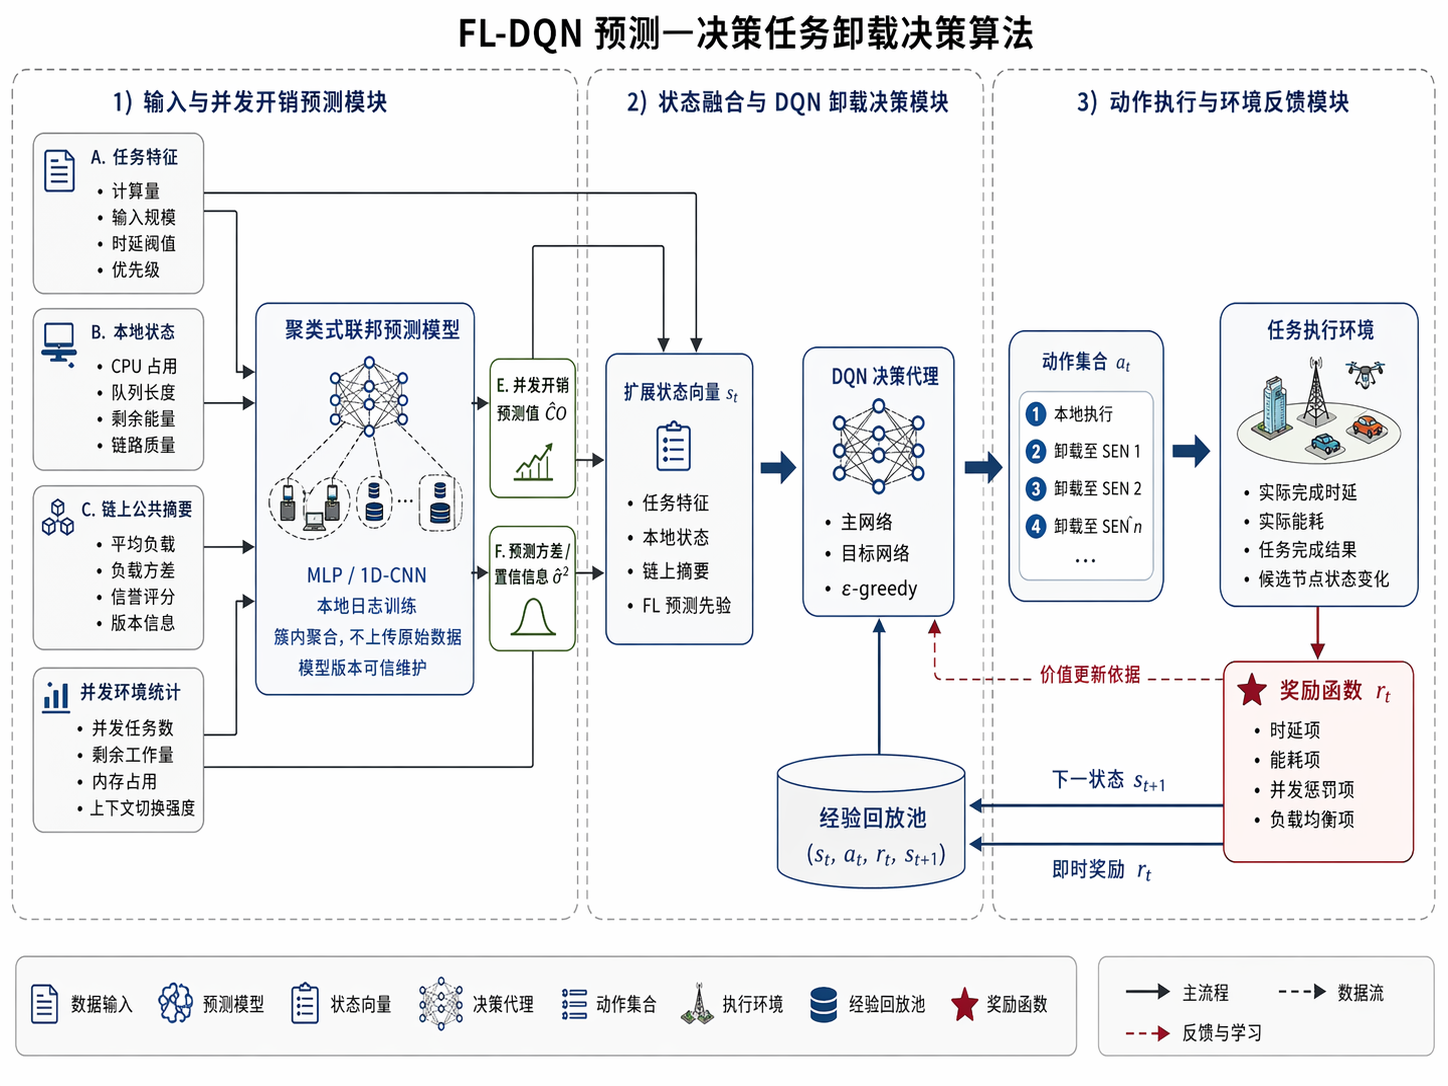
\includegraphics[width=0.96\textwidth]{figures/4-5.png}
    \caption{融合并发开销预测先验的 FL-DQN 在线卸载决策闭环}
    \label{fig:closed_loop}
\end{figure}

这种协同方式的优势在于，它把难以直接编码进解析策略的“未来并发风险”显式注入到了决策模块中。换言之，DQN 并不是在纯粹的即时观测之上做反应式决策，而是在带有预测先验的扩展状态上做前瞻式决策。特别是在高并发、链上状态滞后的场景中，这种差异通常会转化为更低的时延退化斜率和更好的系统鲁棒性。

综合上述设计，FL-DQN 在线卸载决策流程可概括为表~\ref{tab:online_policy} 所示的七个步骤。

\begin{table}[H]
    \centering
    \caption{FL-DQN 在线卸载决策流程}
    \label{tab:online_policy}
    \begin{tabular}{p{1.0cm}p{11.2cm}}
        \toprule
        步骤 & 流程描述                                                        \\
        \midrule
        1  & 终端节点接收新任务，提取计算量、数据大小、任务类型、优先级和截止期等特征。                       \\
        2  & 从本地环境读取 CPU、内存、队列长度、剩余能量与链路状态，并从联盟链获取候选边缘节点的公共摘要。           \\
        3  & 按候选目标节点所属簇调用联邦预测模型，对各候选动作的并发开销和预测不确定性进行快速推理。                \\
        4  & 将任务特征、本地资源状态、链上公共摘要和预测先验拼接为状态向量 $s_t$。                      \\
        5  & DQN 计算各动作的 $Q$ 值，并按 $\varepsilon$-greedy 规则选择本地执行或目标节点卸载动作。 \\
        6  & 环境返回任务完成时延、能耗、并发扰动和完成结果，据此计算奖励并写入经验回放池。                     \\
        7  & 主网络按 mini-batch 更新参数，目标网络按固定步长同步；策略持续与环境交互直至收敛。             \\
        \bottomrule
    \end{tabular}
\end{table}

为了更清楚地展示“预测先验如何进入在线动作选择”，算法~\ref{alg:fldqn_online} 对 FL-DQN 的节点侧执行流程给出伪代码描述。该伪代码与图~\ref{fig:closed_loop} 的区别在于：前者强调实现时的控制流，后者强调预测与决策之间的信息闭环。

\begin{algorithm}[H]
    \caption{FL-DQN 在线任务卸载决策流程}
    \label{alg:fldqn_online}
    \small
    \begin{algorithmic}[1]
        \Statex {输入：}最新可用联邦预测模型 $f_{\theta_f}$，DQN 主网络 $Q(\cdot;\theta_q)$，目标网络 $Q(\cdot;\theta_q^-)$，经验回放池 $\mathcal{B}$。
        \Statex {输出：}收敛后的节点侧卸载策略。
        \For{每个决策周期}
        \State 接收新任务并提取任务特征、本地资源状态与链上公共摘要
        \For{每个候选动作 $a\in\mathcal{A}$}
        \State 构造动作相关特征向量 $\bm{x}(s_t,a)$
        \State 调用 $f_{\theta_f}$ 得到并发开销预测值及不确定性 $\bigl(\widehat{\Delta}_i(s_t,a),\widehat{\sigma}_i^2(s_t,a)\bigr)$
        \EndFor
        \State 拼接得到扩展状态 $s_t$，按 $\varepsilon$-greedy 选择动作 $a_t$
        \State 执行动作并获得即时奖励 $r_t$ 与下一状态 $s_{t+1}$
        \State 将 $(s_t,a_t,r_t,s_{t+1})$ 写入经验回放池 $\mathcal{B}$
        \If{经验池样本数量足够}
        \State 从 $\mathcal{B}$ 随机采样 mini-batch，并按式~(\ref{eq:bellman_target}) 更新主网络
        \State 每隔固定步长同步目标网络参数 $\theta_q^- \leftarrow \theta_q$
        \EndIf
        \EndFor
    \end{algorithmic}
\end{algorithm}

\subsection{算法复杂度与可实现性分析}

对于单次在线决策，若候选边缘节点数量为 $N_c$，预测模型前向推理复杂度为 $\mathcal{O}(P_f)$，Q 网络前向推理复杂度为 $\mathcal{O}(P_q)$，则单次决策复杂度近似为
\begin{equation}
    \mathcal{O}\left(N_c P_f + P_q\right).
\end{equation}
由于 $N_c$ 通常远小于全网节点数，且 $P_f$ 和 $P_q$ 均来自轻量级 MLP/1D-CNN 结构，因此该复杂度满足节点侧实时部署需求。

若考虑训练阶段，则每次 DQN 参数更新需要对一个大小为 $B_q$ 的 mini-batch 执行前向与反向传播，复杂度约为 $\mathcal{O}(B_q P_q)$；经验回放池若容量为 $|\mathcal{B}|$，则其空间复杂度为 $\mathcal{O}(|\mathcal{B}|\,d_s)$，其中 $d_s$ 为状态维度。与引入预测先验所带来的性能收益相比，这部分额外存储开销是可控的。进一步地，预测模型本身可以异步更新，节点侧仅维护最近一次下发的模型副本，因此不会把联邦训练的成本直接叠加到每个在线动作上。

相比之下，若使用中心控制器收集全网细粒度状态再做统一决策，则不仅通信开销更高，而且难以满足天基网络中严格的时延约束。尤其是在链上状态存在确认延迟、候选节点可达性随轨道运动变化的条件下，把所有决策都放在中心完成会进一步放大信息年龄问题，而 FL-DQN 通过“链上摘要 + 本地观测 + 预测先验”的组合，能够在分布式条件下保留较高的动作质量。


\section{实验设计与结果分析}
\label{sec:experiments}

为系统验证所提 FL-DQN 任务卸载方法的有效性，本节按照“预测层验证—端到端性能验证—鲁棒性与可解释性分析—模块贡献分析”的逻辑展开实验。首先，通过并发开销预测精度、训练收敛过程、置信校准结果和异构环境下的预测误差，验证聚类式联邦学习能否为节点侧决策提供可靠的并发风险先验；其次，通过平均任务时延、系统吞吐量、SLA 完成率和 P99 尾时延等指标，分析预测先验是否能够有效转化为实际卸载收益；随后，从链上摘要陈旧性、动作选择偏好和效率--公平性折中三个角度进一步评估方法的鲁棒性与可解释性；最后，通过消融实验分析联邦预测模块、并发惩罚项、经验回放机制和奖励塑形项对整体性能的具体贡献。

需要说明的是，受限于真实在轨天基边缘计算环境难以直接部署和复现实验，本文实验部分采用模型驱动的离散事件仿真方式进行验证。仿真参数依据前文建立的任务层时延模型、能耗模型和并发开销模型设定，并结合图像处理类任务与数值计算类任务构造不同并发强度下的资源竞争场景。实验结果主要用于比较不同策略在相同约束条件下的相对性能差异，而不代表某一具体星载平台的绝对实测性能。

\subsection{实验场景、对比方法与评价指标}
\label{subsec:exp_setup}

实验场景模拟由若干卫星终端 ST、候选卫星边缘节点 SEN、联盟链控制平面和联邦协调单元共同组成的天基分布式计算系统。终端侧任务按照离散事件方式持续到达，每个任务包含计算量、输入数据大小、时延约束、任务类型和优先级等属性；候选边缘节点具有不同的计算能力、队列长度、背景负载和并发任务数；链上公共摘要以固定周期更新，用于提供候选节点的平均负载、负载方差、信誉评分和模型版本信息。为模拟天基网络中的状态滞后现象，实验进一步设置可控的链上摘要延时，并考察不同延时条件下各策略的性能变化。

并发开销预测数据由两类代理任务构造：一类为图像处理任务，用于模拟遥感预处理、轻量识别和视觉感知类边缘负载；另一类为数值计算任务，用于模拟输入规模较小但计算强度较高的计算密集型负载。每条样本记录任务类型、输入规模、估计计算量、节点 CPU 状态、并发任务数、执行中任务剩余工作量、上下文切换强度以及实际完成时延，并根据前文定义的并发开销表达式构造监督标签。这样既能够覆盖数据搬移和计算争用同时存在的混合场景，也能够避免训练样本过度偏向单一任务类型。

对比方法包括以下几类：{FL-DQN} 表示本文提出的完整方法；{DQN-only} 表示不引入联邦预测先验，仅依靠即时状态训练 DQN 策略；{FL-only} 表示使用联邦预测结果辅助启发式卸载，但不进行强化学习策略优化；{Centralized-DQN} 表示在理想条件下能够获得全局实时状态的集中式 DQN，可视为性能上界参考；{Heuristic} 表示基于当前负载、链路质量和队列长度的启发式卸载策略。对于预测层实验，额外比较 {Clustered FL}、{FedAvg}、{Centralized} 和 {Local-only} 四类训练方式，以验证聚类式联邦学习在 Non-IID 数据分布下的优势。

评价指标分为预测层指标和决策层指标。预测层采用 MAE、RMSE 和预测--真实拟合关系衡量并发开销预测精度，同时通过置信校准结果分析模型输出不确定性的有效性。决策层采用平均任务时延、系统吞吐量、SLA 完成率、P99 尾时延、在线决策开销、跨轮次波动和 Jain 公平性指数等指标衡量卸载策略的综合表现。其中，平均任务时延反映整体服务效率，P99 尾时延反映极端拥塞条件下的稳定性，SLA 完成率反映任务时延约束满足能力，Jain 公平性指数用于衡量任务分配在不同候选节点之间的均衡程度。

\subsection{并发开销预测模块性能分析}
\label{subsec:pred_results}

节点侧卸载策略能否提前规避潜在拥塞，很大程度上取决于并发开销预测模块是否能够提供稳定可靠的风险先验。因此，本节首先对预测模块进行独立验证。图~\ref{fig:pred_perf_enhanced} 从联邦训练收敛过程、预测--真实散点密度、置信度校准结果以及不同异构强度下的测试误差四个角度展示了并发开销预测模块的综合性能。

\begin{figure}[H]
    \centering
    
\includegraphics[width=0.97\textwidth]{images/4-new-6.pdf}
    \caption{并发开销预测模块的多维性能结果}
    \label{fig:pred_perf_enhanced}
\end{figure}

由图~\ref{fig:pred_perf_enhanced}(a) 可见，随着通信轮次增加，各类训练方式的验证集 MAE 均逐步下降，说明模型能够从历史执行日志中学习并发开销与任务特征、节点状态和资源竞争程度之间的映射关系。其中，Clustered FL 的误差下降速度明显快于 FedAvg 和 Local-only，并且在训练后期达到更低的稳定误差水平。这表明，在节点负载模式和任务分布存在差异的情况下，先根据负载模式进行聚类，再在簇内执行模型聚合，能够有效缓解统一全局模型在多峰分布下的偏移问题。

图~\ref{fig:pred_perf_enhanced}(b) 给出了预测并发开销与真实并发开销之间的散点密度关系。大多数样本集中分布在对角线附近，说明预测值与真实值总体保持较高一致性。当真实并发开销较低时，样本分布相对紧凑，预测误差较小；当真实并发开销增大时，散点分布略有扩散，说明高并发条件下资源争用的不确定性更强，但整体仍能保持较好的趋势跟踪能力。该结果说明，预测模型不仅能够学习平均意义上的并发开销变化，也能够对不同负载区间下的风险差异做出有效区分。

图~\ref{fig:pred_perf_enhanced}(c) 展示了预测不确定性与实际绝对误差之间的关系。可以看到，经验误差总体随预测不确定性增加而上升，说明模型输出的置信信息具有一定校准意义。换言之，当预测模型对某些样本给出较高不确定性时，这些样本通常也更容易产生较大的实际误差。该结果对于后续 DQN 决策具有重要意义：DQN 不仅可以利用并发开销点估计值，还可以利用不确定性信息判断当前预测是否可靠，从而避免在高风险、高不确定性状态下过度依赖单一预测值。

图~\ref{fig:pred_perf_enhanced}(d) 进一步比较了不同数据异构强度下的测试集 MAE。可以看出，在 IID 场景下，各方法之间的差距相对有限；但随着数据分布从轻度 Non-IID 增强到重度 Non-IID，FedAvg 和 Local-only 的误差增长更为明显，而 Clustered FL 的误差上升幅度较小，表现出更好的异构鲁棒性。该现象说明，标准 FedAvg 在节点负载模式差异较大时容易受到全局平均效应影响，而聚类式联邦学习能够通过簇内聚合保留局部负载特征，从而为节点侧决策提供更加稳定的并发风险估计。

综合图~\ref{fig:pred_perf_enhanced} 的结果可以看出，聚类式联邦学习不仅提高了并发开销预测精度，也提升了模型在异构环境下的收敛稳定性和置信表达能力。这为后续 FL-DQN 将预测先验引入状态空间和奖励函数提供了基础支撑。

\subsection{不同并发强度下的端到端卸载性能分析}
\label{subsec:e2e_results}

在验证并发开销预测模块能够提供有效风险先验之后，进一步需要回答的问题是：预测得到的并发风险信息能否真正转化为任务级卸载性能提升。为此，本文在不同平均并发任务数下，对 FL-DQN 与多种基线方法在平均任务时延、系统吞吐量、SLA 完成率和 P99 尾时延四项指标上的表现进行对比，结果如图~\ref{fig:service_quality} 所示。

\begin{figure}[H]
    \centering
    
\includegraphics[width=0.97\textwidth]{images/4-new-7.pdf}
    \caption{不同并发强度下的卸载决策性能与稳定性}
    \label{fig:service_quality}
\end{figure}

为了进一步给出典型并发区间下的定量对比，表~\ref{tab:e2e_performance_summary} 汇总了低并发、中并发和高并发条件下各方法的关键指标。其中，$\bar{k}$ 表示平均并发任务数，Avg. Delay 表示平均任务时延，Thr. 表示系统吞吐量，SLA 表示 SLA 完成率，P99 表示尾部时延。表中红色表示最优结果，蓝色表示次优结果。需要指出的是，Centralized-DQN 假设能够获得全局实时状态，因此主要作为理想性能上界；FL-DQN 则是在分布式、状态滞后和隐私受限条件下可部署的节点侧策略。

\begin{table*}[t]
    \centering
    \footnotesize
    \caption{不同并发强度下各卸载策略的端到端性能汇总}
    \label{tab:e2e_performance_summary}
    \setlength{\tabcolsep}{2.0mm}
    \renewcommand{\arraystretch}{1.15}
    \resizebox{\linewidth}{!}{
        \begin{tabular}{l|cccc|cccc|cccc}
            \toprule
            \rowcolor{gray!10}
            \multirow{2}{*}{方法}
             & \multicolumn{4}{c|}{低并发 $\bar{k}=4$}
             & \multicolumn{4}{c|}{中并发 $\bar{k}=8$}
             & \multicolumn{4}{c}{高并发 $\bar{k}=12$}                                                       \\
            \rowcolor{gray!10}
             & Avg. Delay $\downarrow$              & Thr. $\uparrow$ & SLA $\uparrow$ & P99 $\downarrow$
             & Avg. Delay $\downarrow$              & Thr. $\uparrow$ & SLA $\uparrow$ & P99 $\downarrow$
             & Avg. Delay $\downarrow$              & Thr. $\uparrow$ & SLA $\uparrow$ & P99 $\downarrow$ \\
            \midrule
            Heuristic
             & 160                                  & 53              & 93.9           & 253
             & 240                                  & 40              & 82.3           & 399
             & 361                                  & 28              & 65.6           & 612              \\

            DQN-only
             & 145                                  & 56              & 95.5           & 228
             & 222                                  & 44              & 86.9           & 368
             & 334                                  & 32              & 72.3           & 548              \\

            FL-only
             & 141                                  & 57              & 96.2           & 219
             & 208                                  & 48              & 89.3           & 331
             & 296                                  & 36              & 77.1           & 489              \\

            FL-DQN
             & \cellcolor{secondcolor}{134}
             & \cellcolor{secondcolor}{59}
             & \cellcolor{secondcolor}{97.3}
             & \cellcolor{secondcolor}{211}
             & \cellcolor{secondcolor}{188}
             & \cellcolor{secondcolor}{52}
             & \cellcolor{secondcolor}{93.1}
             & \cellcolor{secondcolor}{284}
             & \cellcolor{secondcolor}{256}
             & \cellcolor{secondcolor}{43}
             & \cellcolor{secondcolor}{84.7}
             & \cellcolor{secondcolor}{401}                                                        \\

            Centralized-DQN
             & \cellcolor{bestcolor}{130}
             & \cellcolor{bestcolor}{61}
             & \cellcolor{bestcolor}{97.7}
             & \cellcolor{bestcolor}{202}
             & \cellcolor{bestcolor}{181}
             & \cellcolor{bestcolor}{54}
             & \cellcolor{bestcolor}{94.0}
             & \cellcolor{bestcolor}{273}
             & \cellcolor{bestcolor}{247}
             & \cellcolor{bestcolor}{46}
             & \cellcolor{bestcolor}{86.5}
             & \cellcolor{bestcolor}{387}                                                          \\
            \bottomrule
        \end{tabular}}
\end{table*}

由图~\ref{fig:service_quality}(a) 可见，随着平均并发任务数增加，所有方法的平均任务时延均呈上升趋势。这是因为并发任务增多后，候选节点内部的 CPU 时间片争用、缓存冲突、内存带宽竞争和 I/O 排队现象更加明显，导致任务端到端完成时间持续增加。然而，不同方法的时延增长斜率存在明显差异。Heuristic 和 DQN-only 在高并发区间时延上升较快，说明仅依赖当前负载或即时观测状态难以准确判断候选节点的未来拥塞风险。相比之下，FL-DQN 的时延增长更为平缓，说明引入并发开销预测先验后，策略能够在任务卸载前提前识别潜在拥塞节点，从而减少将任务发送到“表面空闲但实际竞争严重”节点的概率。

从表~\ref{tab:e2e_performance_summary} 也可以看出，在低并发、中并发和高并发三个典型场景下，Centralized-DQN 在多数指标上取得最优结果，这是因为其具备理想化的全局实时状态信息，能够作为性能上界参考。而 FL-DQN 在所有典型并发强度下均取得次优结果，并明显优于 DQN-only、FL-only 和 Heuristic。尤其在高并发条件下，FL-DQN 的平均时延为 256 ms，明显低于 DQN-only 的 334 ms 和 Heuristic 的 361 ms；其 SLA 完成率为 84.7\%，也显著高于 DQN-only 和 Heuristic。这说明在分布式可部署约束下，FL-DQN 能够较好逼近集中式策略的性能上界。

图~\ref{fig:service_quality}(b) 给出了系统吞吐量随并发强度变化的情况。随着并发任务数增加，各方法吞吐量均出现不同程度下降，这是由于节点队列积压和任务执行时间延长降低了单位时间内的任务完成数量。Centralized-DQN 由于假设能够获得全局实时状态，因此整体吞吐量最高。FL-DQN 虽略低于 Centralized-DQN，但明显优于 DQN-only、FL-only 和 Heuristic，说明在不依赖全局实时透明信息的前提下，所提方法通过“链上摘要 + 本地观测 + 联邦预测先验”的组合，已经能够获得接近集中式策略的任务处理能力。

图~\ref{fig:service_quality}(c) 展示了 SLA 完成率随并发强度变化的趋势。在低并发条件下，各方法之间的差距相对较小，说明系统资源较充足时，不同策略都较容易满足任务时延约束。但当平均并发任务数持续增加后，Heuristic 和 DQN-only 的完成率下降更快，表明其在高负载条件下更容易产生拥塞误判和任务超时。FL-DQN 的 SLA 完成率下降最慢，说明其能够通过预测先验提前规避高风险卸载动作，从而在资源竞争增强时仍保持较高的任务完成质量。

图~\ref{fig:service_quality}(d) 从尾部性能角度进一步验证了上述结论。P99 尾时延反映了最差一部分任务的完成情况，对时延敏感型天基业务尤为重要。随着并发任务数增加，各方法的 P99 尾时延均明显上升，但 FL-DQN 的增长幅度相对较小。相比 DQN-only 和 Heuristic，FL-DQN 在高并发区间能够显著降低尾部时延，说明其不仅改善了平均意义上的服务质量，也有效抑制了极端拥塞样本对系统稳定性的影响。

总体来看，图~\ref{fig:service_quality} 和表~\ref{tab:e2e_performance_summary} 共同表明，FL-DQN 的优势在中高并发场景中更加明显。这与本文方法设计目标一致：当系统处于轻载状态时，候选节点之间的资源竞争尚不显著，预测模块带来的收益有限；而当系统逐步逼近拥塞边界时，并发开销预测能够为 DQN 提供更有价值的前瞻信息，使策略在平均时延、吞吐量、SLA 完成率和尾部时延方面均表现出更好的稳定性。
\subsection{鲁棒性、动作偏好与多目标折中分析}
\label{subsec:robustness_results}

仅从平均时延或完成率角度评价卸载策略，仍不足以全面说明方法的可部署性。天基网络中链路窗口有限、链上摘要存在确认延迟，节点状态不可避免地具有陈旧性；同时，卸载策略还应具备可解释的动作选择行为，并在效率、能耗和节点均衡之间取得合理折中。基于此，本文进一步从链上陈旧性敏感性、动作选择偏好和效率--公平性折中三个角度进行分析，结果如图~\ref{fig:robustness_tradeoff} 所示。

\begin{figure}[H]
    \centering
    
\includegraphics[width=0.88\textwidth]{images/4-new-8.pdf}
    \caption{鲁棒性、动作偏好与多目标折中结果}
    \label{fig:robustness_tradeoff}
\end{figure}

图~\ref{fig:robustness_tradeoff}(a) 展示了链上摘要延时增加时各方法的平均任务时延变化。可以看到，随着链上摘要延时从较低水平逐步增加，各方法的平均时延均有所上升。这是因为候选节点公共摘要越陈旧，终端侧获得的节点负载状态越可能偏离真实运行状态，从而增加错误卸载的概率。然而，FL-DQN 的退化幅度明显小于 DQN-only、FL-only 和 Heuristic。该结果说明，FL-DQN 并不完全依赖链上摘要本身，而是能够通过本地实时观测和联邦预测模型对状态陈旧性进行一定补偿。当链上信息不能准确反映当前节点状态时，预测模块仍可根据历史负载模式和并发环境特征估计潜在风险，从而降低摘要延迟对决策质量的影响。

图~\ref{fig:robustness_tradeoff}(b) 给出了 FL-DQN 在不同候选节点负载风险区间下的动作选择热力图。该热力图通过统计策略收敛后在测试集中的动作选择频次，并对同一风险区间内的动作次数进行归一化得到。可以看出，在负载风险较低时，策略更倾向于选择本地执行或风险较低的候选边缘节点；随着候选节点负载风险逐步升高，动作选择概率逐渐向其他节点分散，表明智能体会根据风险变化动态调整卸载目标，而不是长期固定选择某一个高性能节点。该结果说明，FL-DQN 学到的并不是简单的“选择当前负载最低节点”规则，而是一种结合任务属性、链上摘要和并发风险预测的自适应卸载行为。

图~\ref{fig:robustness_tradeoff}(c) 进一步展示了不同方法在能时积 EDP 与 Jain 公平性指数之间的折中关系，其中气泡大小表示对应方法的任务完成率。EDP 越低，说明方法在时延和能耗之间具有更好的综合效率；Jain 公平性指数越高，说明任务在不同节点之间分配越均衡。可以看到，Centralized-DQN 由于拥有理想全局状态，在公平性和效率方面表现较好，但其依赖强全局实时信息假设，实际部署难度较高。FL-DQN 在 EDP 和公平性之间取得了较优折中，虽然其公平性略低于集中式上界，但明显优于 DQN-only、FL-only 和 Heuristic，并且仍保持较高任务完成率。相比之下，Heuristic 和 DQN-only 更容易将任务集中到少数表面负载较低的节点，从而导致公平性下降和能时积增大。

综合图~\ref{fig:robustness_tradeoff} 可以看出，FL-DQN 的优势不仅体现在平均性能指标上，还体现在对链上状态滞后的适应能力、动作选择行为的合理性以及效率--公平性多目标折中能力上。这说明所提方法更符合天基分布式计算环境中“信息不完全、状态有时滞、节点负载动态变化”的实际部署需求。

\subsection{消融实验与模块贡献分析}
\label{subsec:ablation_results}

为了进一步分析完整方法中各组成模块的具体作用，本文设计消融实验，分别移除联邦预测模块、并发惩罚项、经验回放机制和奖励塑形项，并与完整 FL-DQN 进行对比。除被移除模块外，其余训练参数、任务到达过程、候选节点配置和评价指标均保持一致，以保证不同消融版本之间具有可比性。为便于直接对比，表~\ref{tab:ablation_summary} 汇总了平均并发任务数为 $16$ 时的关键指标，其中 Avg. Delay 和 SLA 分别来自图~\ref{fig:ablation_results}(a)(b) 的高并发点，Online Cost 与 Std. Dev. 则对应图~\ref{fig:ablation_results}(c) 的双纵轴柱状统计结果。表中红色表示最优结果，蓝色表示次优结果。

\begin{table}[H]
    \centering
    \footnotesize
    \caption{FL-DQN 各模块消融实验结果}
    \label{tab:ablation_summary}
    \setlength{\tabcolsep}{2.3mm}
    \renewcommand{\arraystretch}{1.18}
    \begin{tabular}{lccccp{3.1cm}}
        \toprule
        \rowcolor{gray!10}
        方法变体
         & Avg. Delay $\downarrow$
         & SLA $\uparrow$
         & Online Cost $\downarrow$
         & Std. Dev. $\downarrow$
         & 结果说明                                 \\
        \midrule
        FL-DQN
         & \cellcolor{bestcolor}{209}
         & \cellcolor{bestcolor}{91.2}
         & 3.8
         & \cellcolor{bestcolor}{5.1}
         & 完整方法，综合性能最优                          \\

        -FL 预测
         & 284
         & 80.1
         & \cellcolor{secondcolor}{3.1}
         & 9.6
         & 缺少并发风险先验，退化最明显                       \\

        -并发惩罚
         & 243
         & 84.7
         & 3.6
         & 8.1
         & 拥塞规避约束减弱                             \\

        -经验回放
         & 256
         & 86.4
         & \cellcolor{bestcolor}{2.4}
         & 11.2
         & 开销最低但训练波动最大                          \\

        -奖励塑形
         & \cellcolor{secondcolor}{238}
         & \cellcolor{secondcolor}{87.9}
         & 3.4
         & \cellcolor{secondcolor}{7.3}
         & 收敛引导能力减弱                             \\
        \bottomrule
    \end{tabular}
\end{table}

进一步地，图~\ref{fig:ablation_results} 从平均时延、SLA 完成率以及“在线决策开销--跨轮次波动”联合视角展示了消融实验结果。为了便于排版，图~\ref{fig:ablation_results} 由三个子图组合而成。

\begin{figure}[H]
    \centering
    \begin{subfigure}[t]{0.48\textwidth}
        \centering
        
\includegraphics[width=\linewidth]{chapter4_5_fldqn_package/figures/fig4_9_a_avg_delay_cn.pdf}
        \caption{平均时延随并发度变化}

    \end{subfigure}
    \hfill
    \begin{subfigure}[t]{0.48\textwidth}
        \centering
        
\includegraphics[width=\linewidth]{chapter4_5_fldqn_package/figures/fig4_9_b_sla_cn.pdf}
        \caption{SLA 完成率随并发度变化}

    \end{subfigure}

    \vspace{0.25cm}
    \begin{subfigure}[t]{0.90\textwidth}
        \centering
        
\includegraphics[width=\linewidth]{chapter4_5_fldqn_package/figures/fig4_9_c_overhead_variance_cn.pdf}
        \caption{在线决策开销与跨轮次波动联合对比}

    \end{subfigure}
    \caption{消融实验结果}
    \label{fig:ablation_results}
\end{figure}

图~\ref{fig:ablation_results}(a) 展示了不同消融版本在平均并发任务数增加时的平均时延变化。可以看到，完整 FL-DQN 在所有并发水平下均保持最低平均时延；去除 FL 预测模块后，平均时延显著上升，且并发任务数越高，性能劣化越明显。这说明联邦预测模块是完整方法取得性能优势的核心来源。没有预测先验时，DQN 只能依赖当前观测状态和链上摘要进行反应式决策，难以及时识别候选节点的潜在并发风险，因此在高并发条件下更容易发生错误卸载。相比之下，去除并发惩罚项后时延也有所增加，但劣化程度低于去除 FL 预测模块，说明并发惩罚主要起到强化拥塞规避偏好的作用，而预测模块则决定了策略是否具备风险前瞻能力。

图~\ref{fig:ablation_results}(b) 给出了不同消融版本的 SLA 完成率变化趋势。完整 FL-DQN 的完成率始终最高，并且随着并发增强下降较为平缓；去除 FL 预测模块后，SLA 完成率下降最明显，说明缺少并发风险估计会直接影响任务是否能够在时延阈值内完成。去除并发惩罚项后，SLA 完成率也明显低于完整方法，表明仅将预测值作为状态输入仍不足以完全引导策略规避拥塞，还需要在奖励函数中显式体现并发开销代价，使智能体在训练过程中形成对高风险动作的惩罚记忆。

图~\ref{fig:ablation_results}(c) 以双纵轴柱状图联合比较了各版本的在线决策开销与跨轮次波动。完整 FL-DQN 的在线开销略高于去除 FL 预测模块或去除经验回放的简化版本，这是因为完整方法需要在决策前调用预测模型，并进行 DQN 动作价值计算；但其开销仍维持在毫秒级，满足节点侧实时决策需求。与此同时，完整 FL-DQN 的跨轮次标准差最低，说明其在多次独立运行中更稳定。去除经验回放后尽管在线开销最低，但这往往以更大的跨轮次波动为代价；去除 FL 预测模块后波动同样明显增大，说明缺少稳定风险先验会降低策略一致性。该联合结果表明，完整方法在“决策效率--训练稳定性”之间取得了更优综合折中。



综合消融实验结果可以看出，FL 预测模块决定了策略的风险前瞻能力，是降低高并发时延和维持 SLA 完成率的关键；并发惩罚项增强了策略对拥塞节点的规避倾向，使预测信息能够更直接地转化为优化目标；经验回放机制主要提升训练稳定性，降低跨轮次波动；奖励塑形项则进一步改善策略收敛方向和任务完成质量。因此，完整 FL-DQN 的性能提升并非来自单一模块堆叠，而是来自预测先验、奖励约束和强化学习稳定机制之间的协同作用。

\subsection{本节小结}
\label{subsec:exp_summary}

本节围绕并发感知任务卸载方法的有效性进行了分层实验验证。预测层结果表明，聚类式联邦学习能够在不集中上传原始日志的前提下，有效学习候选节点的并发开销变化规律，并在 Non-IID 环境下保持较好的预测精度和收敛稳定性。端到端卸载结果表明，将并发开销预测值及其置信信息引入 DQN 后，节点侧策略在平均任务时延、系统吞吐量、SLA 完成率和 P99 尾时延等指标上均优于分布式基线方法，尤其在中高并发区间优势更加明显。鲁棒性分析进一步说明，FL-DQN 能够在链上摘要存在陈旧性的情况下维持较平缓的性能退化，并形成符合风险变化规律的动作选择行为。消融实验则验证了联邦预测模块、并发惩罚项、经验回放机制和奖励塑形项对整体性能提升的不同贡献。

总体而言，实验结果说明，本文所提出的 FL-DQN 方法能够在隐私受限、状态滞后和负载异构的天基分布式计算环境中，将联邦学习得到的并发风险预测有效转化为节点侧实时卸载决策收益，从而在时延、吞吐量、完成率、尾部稳定性和负载均衡之间取得更合理的综合折中。

\section{本章小结}
\label{sec:chapter4_conclusion}

本章围绕天基网络任务层实时卸载问题，提出了一个面向并发开销的“联邦预测 + DQN 决策”闭环方法。不同于第三章从系统层讨论全局可信协同资源分配，本章进一步下沉到节点侧，以单任务到达瞬间的快速动作选择为核心，系统性解决了链上状态滞后、隐私受限、负载动态变化和并发资源竞争等多重挑战，因此在全文中承担着把“可信共享能力”转化为“实时执行能力”的桥梁作用。

具体而言，本文首先从任务层视角建立了时延、能耗与并发开销的统一代价模型，并给出了并发开销的形式化定义、工程近似表达及其可分解解释；随后，针对节点本地日志难以集中上传且样本分布高度异构的问题，构建了分层聚类联邦学习框架，实现并发开销预测模型的隐私友好训练；进一步地，本文将预测值及其置信信息显式纳入 DQN 状态空间，并通过并发代价约束、不确定性惩罚和负载均衡惩罚影响奖励反馈，使卸载策略具备对潜在并发风险的前瞻感知能力。实验结果表明，在中等并发工作点 $\bar{k}=8$ 下，所提 FL-DQN 相比 DQN-only 的平均任务时延下降约 $15.3\%$、P99 时延下降约 $22.8\%$、吞吐量提升约 $18.2\%$、SLA 完成率提高约 $6.2$ 个百分点；在高并发工作点 $\bar{k}=12$ 下，其优势进一步扩大，并在链上状态滞后条件下保持更平缓的性能退化趋势。

归纳而言，本章形成了以下三个结论：第一，并发开销是影响天基网络任务级卸载质量的关键隐藏变量，不能被简单平均负载替代；第二，聚类式联邦学习能够在不上传原始数据的前提下有效建模并发风险，为节点侧决策提供可靠先验；第三，将预测先验与强化学习决策进行深度耦合，能够显著增强策略在信息不完全与高并发场景下的鲁棒性。由此，第三章所建立的系统层可信协同框架与本章提出的任务层实时决策机制共同构成了一个跨层闭环：前者保障状态共享的可信与可得，后者保障任务执行的高效与稳健。上述研究也为后续进一步讨论跨层协同优化、多智能体联合决策或更复杂的星地协同边缘智能机制奠定了方法基础。
